\section{Introducere}
Programele cu mai multe fire de execuție au devenit mult mai comune
în programarea modernă. Procesoarele noi și plăcile grafice conțin mai
multe nuclee separate și capabilități de virtualizare, iar pentru a
folosi eficient aceste resurse, programele axate pe performanță
partajează sarcinile pe care le au de îndeplinit în mai multe fire de
execuție ce pot fi executate în paralel pe același hardware.

Dar prin introducerea acestui nou model de programare, s-a introdus și o
nouă gamă de dificultăți și posibilități de a face greșeli programatice.
Firele de execuție dintr-un proces accesează același spațiu de memorie
RAM, același disc, același monitor și alte dispozitive ale
calculatorului. De pildă dacă mai multe fire de execuție ce rulează
\textit{concurent} încearcă să stocheze informații diferite la aceeași
adresă de memorie RAM, rezultatul obținut nu este clar definit.
Problemele de acest tip se rezolvă folosind
\textit{mecanisme de sincronizare} pentru a controla și arbitra accesul
la resurse comune pe care mai multe fire de execuție le folosesc
concurent. Majoritatea acestor mecanisme sunt construite în jurul unor
\textit{primitive de sincronizare} printre care se numără
\textit{mutex}, \textit{semaphore}, \textit{read-write lock} și
\textit{condition variable}.

Folosirea acestor primitive este considerată dificilă. Orice resursă
partajată care este accesată concurent de mai multe fire de
execuție poate duce la un \textit{race condition} (o situație în care
rezultatul este nepredictibil pentru că depinde de ordinea în care
firele de execuție accesează resursa, dar de cele mai multe ori nu este
cel intenționat), așa că toate situațiile de acest tip din program
trebuie apărate folosind mecanisme de sincronizare. În același timp,
orice exces de astfel de mecanisme poate duce la alte tipuri de erori
cum ar fi \textit{deadlock} (situație în care două sau mai multe fire de
execuție se blochează reciproc, și niciuna nu mai poate progresa),
\textit{starvation} (un fir nu mai ajunge niciodată să își îndeplinească
sarcina pentru că nu mai primește acces la resursa partajată) sau
degradarea performanței programului (deoarece principalul motiv pentru
care se folosesc mai multe fire de execuție este performanța, aceasta
este de multe ori la fel de importantă ca și corectitudinea).

Dificultatea de înțelegere și utilizare a acestor concepte, împreună cu
rezultatele dezastruoase care apar frecvent din cauza erorilor de
programare crează o nevoie de unelte care să ajute dezvoltatorii de
aplicații în a identifica și repara acest tip de greșeli. Deși există
deja multe astfel de unelte în ecosistemul programării, nu toate
problemele ce pot apărea sunt rezolvate de unelte existente. De
asemenea, fiecare program care folosește aceste primitive de
sincronizare are alte nevoi, și o unealtă generică de multe ori nu poate
rezolva problemele specifice întâmpinate de un anumit program.

Vom prezenta în continuare un proiect ce are ca scop nu doar crearea
unei astfel de unelte, ci a unei platforme de dezvoltare ce facilitează
conceperea și implementarea de unelte noi și specifice unei anumite
nevoi printr-un efort minim.

\subsection{SyncAnalysis}
\textit{SyncAnalysis} este un proiect ce își propune crearea unui sistem
în care este ușor de dezvoltat unelte noi de diagnosticare a problemelor
ce pot apărea în folosirea mecanismelor primitive de sincronizare (și nu
doar).

Ideea din spatele acestui proiect vine din următoarea observație:
prin capturarea unor evenimente cheie pe parcursul execuției unui
program, se pot diagnostica o gamă largă de probleme pe care le
întâmpină acesta. Un exemplu simplu ar fi că prin observarea tuturor
cererilor de \textit{lock} și \textit{unlock} pe o instanță de
\textit{mutex}, se poate observa că \textit{mutex}-ul respectiv nu este
necesar dacă toate apelurile se întâmplă în contextul aceluiași fir de
execuție.

Din această observație se vede că proiectul folosește strategia
\textit{post-mortem} pentru analiza programelor: de-a lungul execuției
programului se înregistrează evenimentele de interes, pentru a fi
procesate și analizate separat după terminarea acestuia. Această
strategie a fost aleasă pentru că nu este deloc intrusivă: necesită
schimbări minime sau nule în codul sursă al programului (în anumite
situații nu necesită nici recompilarea codului sursă al unui
program) și nu degradează prea tare performanța programului în sine
pentru a face analiza. Alte strategii de analiză folosite în unelte
existente includ analiză \textit{on-the-fly}, în care analiza este
făcută în paralel cu execuția programului în același proces, precum în
ThreadSanitizer\cite{ThreadSanitizer} și analiză \textit{statică}, în
care codul sursă în sine este analizat, nu programul obținut prin
compilare, precum în Clang Thread Safety Analysis
\cite{ClangThreadSafetyAnalysis}.

Se distinge astfel direcția generală a acestui sistem. Prima și cea mai
importantă componentă este o bibliotecă ce înregistrează evenimentele
interesante în timpul execuției programului și le serializează într-un
fișier, pentru a fi analizate separat de alt program. Detalii despre
această bibliotecă și implementarea ei se găsesc în secțiunea
\textbf{\ref{library}}.

După execuția programului client obținem o colecție de evenimente,
capturate și serializate eficient într-un fișier cu ajutorul
bibliotecii descrise mai sus. În continuare, trebuie făcută o analiză
a acestor evenimente, iar proiectul oferă o soluție pentru asta în forma
unui program independent numit \lstinline{SyncAnalysis}. Acest program,
precum biblioteca de capturare a evenimentelor, este unul de uz general,
și nu este direct legat de analiza primitivelor de sincronizare. Acesta
nu execută pe cont propriu nicio analiză asupra evenimentelor, ci se
bazează pe o suită de module separate numite \textit{analizori}. Acești
analizori sunt distribuiți sub formă de biblioteci dinamice pe care
\lstinline{SyncAnalysis} le încarcă la începutul execuției. Programul se
ocupă de a deserializa și indexa evenimentele din fișier în memorie,
pentru ca apoi \textit{analizorii} să diagnosticheze erori, avertismente
sau în general informații utile pe baza acestor evenimente, iar
programul să creeze și să afișeze apoi rapoarte pentru utilizator. Mai
multe detalii despre acest program se găsesc în secțiunea
\textbf{\ref{executable}}, iar despre analizorii implementați ca exemplu
pentru analiza primitivelor de sincronizare în secțiunea
\textbf{\ref{analyzers}}.

Biblioteca și programul de analiză post-mortem sunt de uz general,
neavând în mod direct o interfață specifică analizării primitivelor de
sincronizare. De aceea proiectul conține și două exemple de biblioteci
pentru a facilita folosirea bibliotecii de capturare a evenimentelor în
scopul de analiză a primitivelor de sincronizare, descrise în detaliu în
Secțiunea \textbf{\ref{integration-libraries}}.

În Figura \ref{fig:architecture} se poate vedea arhitectura software a
proiectului SyncAnalysis. Cu albastru sunt marcate elementele de uz
general, adică cele independente de unealta dezvoltată (folosibile chiar
pentru unelte care nu se ocupă de analiza primitivelor de sincronizare),
cu verde sunt marcate elementele ce sunt specifice unei anumite unelte,
iar cu gri sunt marcate elementele programului client.

\begin{figure}[ht]
\centering
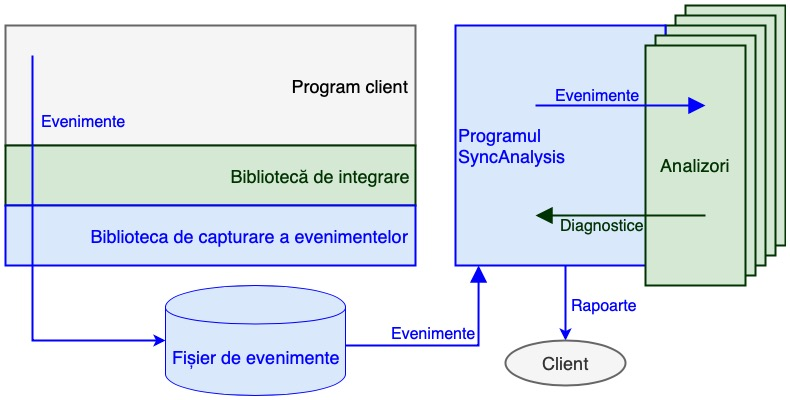
\includegraphics[width=14cm]{architecture.jpg}
\caption{Arhitectura proiectului SyncAnalysis}
\label{fig:architecture}
\end{figure}

\subsection{Comparație cu ThreadSanitizer}
O unealtă populară ce ajută la diagnosticarea folosirii insuficiente a
mecanismelor de sincronizare este ThreadSanitizer\cite{ThreadSanitizer}.
Folosirea acestuia implică compilarea programului cu un compilator care
implementează suport pentru ThreadSanitizer, folosind opțiunile de linie
de comandă documentate de compilator (de exemplu, pentru Clang pe Linux
opțiunea este \lstinline{-fsanitize=thread}). Executabilul obținut prin
compilare verifică toate scrierile în memoria RAM și emite erori dacă
o scriere este concurentă cu o alta sau cu o citire, și cele două nu
sunt explicit sincronizate.

În Fragmentul de cod \ref{code:thread-sanitizer} (parafrazat din site-ul
oficial de documenție al proiectului \cite{ThreadSanitizerDoc}) se vede
cum ThreadSanitizer analizează programul \textit{on-the-fly}: analiza
este făcută direct în cadrul execuției programului, în același proces.
Asta duce la o încetinire drastică a programului și la un consum ridicat
de memorie. Măsurătorile făcute pentru articolul \cite{ThreadSanitizer}
arată o creștere a timpului de execuție între 120\% și 2760\%, și în
consumul de memorie între 20\% și 660\%, în funcție de programul
analizat.

\begin{lstlisting}[caption=Exemplu de folosire ThreadSanitizer,
                   label=code:thread-sanitizer]
% clang -fsanitize=thread -g -O1 -o program tiny_race.c
% ./program
WARNING: ThreadSanitizer: data race (pid=19219)
  Write of size 4 at 0x7fcf by thread T1:
    #0 Thread1 tiny_race.c:4 (exe+0xa360)
  Previous write of size 4 at 0x7fcf by main thread:
    #0 main tiny_race.c:10 (exe+0xa3b4)
  Thread T1 (running) created at:
    #0 pthread_create tsan_interceptors.cc:705 (exe+0xc790)
    #1 main tiny_race.c:9 (exe+0xa3a4)
\end{lstlisting}

De asemenea, ThreadSanitizer are nevoie de ajutor din partea
compilatorului, deci poate fi folosit doar cu compilatoare ce
încorporează explicit suport pentru el. Deși această unealtă este
folosită în companii mari din industrie \cite{ThreadSanitizer}, aceste
dezavantaje îl fac inutilizabil pentru anumite proiecte obligate să
folosească un anumit compilator care nu suportă ThreadSanitizer sau
care sunt executate în contexte unde reducerea drastică a performanței
nu este fezabilă nici măcar pentru teste sau simulări.

Prin comparație, o unealtă construită folosind proiectul SyncAnalysis
face analiza evenimentelor \textit{post-mortem}, și prin urmare nu duce
la creșteri atât de mari în consumul de timp sau memorie în timpul
execuției programului. În schimb fișierele de evenimente pot deveni
destul de mari dacă programul analizat este executat mult timp sau
capturează multe tipuri de evenimente.

\subsection{Comparație cu Clang-Tidy}
\textit{Clang-Tidy}\cite{ClangTidy} este o unealtă ce efectuează analiză
\textit{statică} asupra codului sursă a unui proiect. Deoarece analiza
se face static, fără a necesita execuția programului în sine,
considerentele de performanță a programului sunt inexistente: programul
compilat nu se schimbă din cauza folosirii uneltei, deci nu se aplică
problema de o degradare a performanței sau o creștere a resurselor
folosite din niciun punct de vedere.

Deși accentul nu este pus pe folosirea corectă sau eficientă a
primitivelor de sincronizare în cel din urmă, comparația dintre
proiectele \textit{SyncAnalysis} și \textit{Clang-Tidy} este aptă pentru
că amândouă încearcă să creeze un sistem de unelte, mai degrabă decât
să încerce să fie o unealtă de sine stătătoare. \textit{Clang-Tidy}
permite dezvoltatorilor să scrie noi analizori folosind o interfață
elegantă de C++, în care este necesară strict implementarea analizei în
sine, într-un mod declarativ și simplu, programul \lstinline{Clang-Tidy}
rezolvând în spate toate celelalte probleme pentru a duce la o unealtă
completă.

În timp ce proiectul \textit{Clang-Tidy} permite scrierea cu efort mic a
unor analizori statici pentru codul sursă de C și C++,
\textit{SyncAnalysis} face asta pentru analizori \textit{post-mortem}.
